\documentclass{article}
\usepackage[utf8]{inputenc}
\usepackage{amsmath}
\usepackage{braket}
\usepackage{gensymb}
\usepackage{amssymb}
\usepackage{natbib}
\usepackage{graphicx}
\usepackage{listings}
\usepackage{color}
\usepackage{tikz}
\usepackage{multicol}
\usetikzlibrary{arrows}
\usepackage{hyperref}
\hypersetup{
    colorlinks=true,
    linkcolor=blue,
    filecolor=magenta,      
    urlcolor=cyan,
}
\usepackage{float}
\restylefloat{figure}

\usepackage[figurename=Figure]{caption}

\definecolor{codegreen}{rgb}{0,0.6,0}
\definecolor{codegray}{rgb}{0.5,0.5,0.5}
\definecolor{codepurple}{rgb}{0.58,0,0.82}
\definecolor{backcolour}{rgb}{0.95,0.95,0.92}
 
\lstdefinestyle{mystyle}{
    backgroundcolor=\color{backcolour},   
    commentstyle=\color{codegreen},
    keywordstyle=\color{magenta},
    numberstyle=\tiny\color{codegray},
    stringstyle=\color{codepurple},
    basicstyle=\footnotesize,
    breakatwhitespace=false,         
    breaklines=true,                 
    captionpos=b,                    
    keepspaces=true,                 
    numbers=left,                    
    numbersep=5pt,                  
    showspaces=false,                
    showstringspaces=false,
    showtabs=false,                  
    tabsize=2
}
 
\lstset{style=mystyle}
\lstset{
    language=Erlang,
    mathescape=true
}

\title{FYS2140 - Home exam 2018}
\author{Canditate: 15199}
\date{March 2018}

\begin{document}

\maketitle

\section*{Problem 1}

\subsection*{Particle nature of the photon}

\subsubsection*{a1.}


Comptons scattering forumla can be written on the form
\begin{equation}
\Delta \lambda = \lambda_{s} - \lambda_{i} = \lambda_C(1 - \cos{\theta}),
\end{equation}

where $\lambda_{i}$ is the incident photon, $\lambda_{s}$ is the scattered photon, $\cos{\Theta}$ is the angle between the horizontal and the scattered photon, $\lambda_C = h/(m_ec) = 2.43\times 10^{-3}nm$ is the \textit{Compton wavelength for the electron} where $h$ is Plancks constant, $m_c$ is the electron mass and $c$ is the speed of light. Figure 1 shows a schematic of the setup.

\begin{figure}[t]
\centering
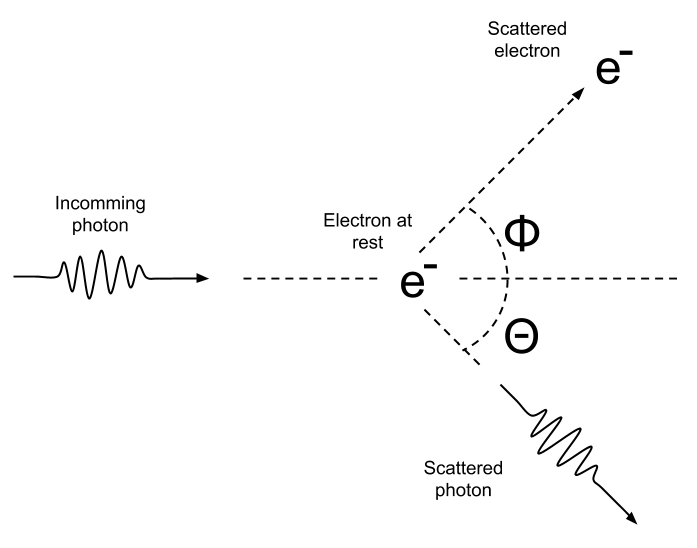
\includegraphics[width=0.6\textwidth]{comptonscattering}
\caption{Compton scattering.}
\label{fig:figure_label}
\end{figure}

\subsubsection*{a2.}

Using Comptons formula, we can find the angle by

\begin{equation}
\Theta = \cos^{-1}{\big( 1 - \frac{\Delta \lambda}{\lambda_C} \big)} = \cos^{-1}{\big(1 - \frac{0.0749 \ nm - 0.0709 \ nm}{0.00243 \ nm} \big)} \approx 130^{\circ},
\end{equation}

which seems like a reasonable result concidering the graphs given in the problem.

\subsubsection*{a3.}

\begin{equation}
\frac{\lambda_C}{\lambda_i}
\end{equation}

Visible light yields wavelengths in the range $380 \ nm - 750 \ nm$. X-rays have shorter wavelengths and thus 
 

\subsection*{Wave nature of the neutron}

\subsubsection*{b1.}

Average energy is given by

\begin{equation}
\braket{E} = \frac{3}{2}k_BT,
\end{equation}

where $T$ is the temperatur in Kelvin and $k_B$ is Boltzmanns constant. $25^\circ = 298K$ and thus

\begin{equation}
\rightarrow \braket{E} = 1.5\times(1.38\times 10^{-23}m^2kgs^{-2}K^{-1})(298.15K) \approx 6.17\times 10^{-21}J.
\end{equation}

Momentum is found from the particles kinetic energy

\begin{equation}
\braket{E} = \frac{1}{2}mv^2 \rightarrow \braket{p} = \sqrt{2\braket{E}m_n},
\end{equation}

where $m_n$ is the neutron mass

\begin{equation}
\rightarrow \braket{p} = \sqrt{1*6.17\times 10^{-21}J\times 1.67\times 10^{-27}kg} \approx 4.54\times 10^{-24}.
\end{equation}

Finally we can find the wavelenth by using the \textit{deBroglie relation} 

\begin{equation}
\lambda = \frac{h}{p} \rightarrow \lambda = \frac{6.32\times 10^{-34}J}{4.54\times 10^{-24}} \approx 1.30\times 10^{-10}m \approx 0.1nm
\end{equation},

where $h$ is Plancks constant.

\subsubsection*{b2.}

\textit{Bragg diffraction} is gi en by

\begin{equation}
n\lambda = 2d\sin{\theta},
\end{equation}

where $n$ is a positive integer and $\lambda$ is the \textit{wavelength of the incident wave}.

Maximum intensity is given at $n=1$, and thus

\begin{equation}
\theta_{max} = \sin^{-1}{\frac{\lambda}{2d}}
\end{equation}

\section*{Problem 2}

\subsection*{Radioactive $\alpha$-decay}

\subsubsection*{a.}

We find $A$ by \textit{normalizing the wavefunction}. $|\Psi(x, 0)| = \Psi^*\Psi$, where $\Psi^*$ is the complex conjugate and thus, the imaginary part will vannish and the integral becomes

\begin{equation}
|\Psi(x, 0)|^2 = |A|^2\int_{-\infty}^{+\infty}e^{-(x-x_0)/2a^2} = 1.
\end{equation}

Substituting $u = x-x_0 \rightarrow du = dx$ and $\lambda = 1/(2\pi a^2)$ yields the following standard integral that can be found in Rottmann

\begin{equation}
|A|^2\int_{-\infty}^{+\infty} e^{-\lambda u} du = |A|^2\sqrt{\frac{\pi}{\lambda}} = |A|^2\sqrt{2\pi a^2} = 1 \rightarrow A = \bigg(\frac{1}{2\pi a^2}\bigg)^{1/4}
\end{equation}

which gives 

\begin{equation}
\Psi(x, 0) = \bigg(\frac{1}{\sqrt{2\pi a^2}}\bigg)^{1/4}e^{-(x-x_0)/4a^2}e^{ikx}
\end{equation}



\subsubsection*{b.}

We need to find general solutions for the three regions for which the particle can exist. As figure 2 shows, we have that $0 \leq E \leq V_0 \rightarrow E > 0$, so we're dealing with \textit{scattering states}.

\bigskip

For $(0 \leq x \leq x_1), \ V(x) = 0$ and the time-independent Schrödinger equation reads

\begin{equation}
-\frac{\hbar^2}{2m}\frac{d^2\psi}{dx^2} = E\psi \rightarrow \frac{d^2\psi}{dx^2} = -k^2\psi, \ \ k \equiv \frac{\sqrt{2mE}}{\hbar}
\end{equation}

which general solution is

\begin{equation}
\psi(x) = Ae^{ikx} + Be^{-ikx}.
\end{equation}

For $(x_1 \leq x \leq x_2), \ V(x) = V_0 \rightarrow E < V_0$, so we will get complex solutions and thus the time-independent Schrödinger equation reads

\begin{equation}
-\frac{\hbar^2}{2m}\frac{d^2\psi}{dx^2} + V_0\psi = E\psi \rightarrow \frac{d^2\psi}{dx^2} = -q^2\psi, \ \ q \equiv i\kappa, \ \kappa \equiv \frac{\sqrt{2m(V_0 - E)}}{\hbar}
\end{equation}

which general solution is

\begin{equation}
\psi(x) = Ce^{iqx} + De^{-iqx} = Ce^{-\kappa x} + De^{\kappa x} \rightarrow Ce^{\kappa x} + De^{-\kappa x}.
\end{equation}

(I switched the constants C and D to make the equation consistant with my scetch.)

For ($x \geq x_2$), the general solution is simular to the left region, however, the latter term in the sum prepresents a wave comming in from the right and thus is omited from the equation

\begin{equation}
\psi(x) = Fe^{ikx}.
\end{equation}

To summarize, the general solution of the three regions are

\begin{equation}
\psi(x) = \begin{cases}
Ae^{ikx} + Be^{-ikx} \ \ &, \ \ 0 \leq x \leq x_1 \\
Ce^{\kappa x} + De^{-\kappa x} \ \ &, \ \ x_1 \leq x \leq x_e \\
Fe^{ikx}  &, \ \ x \geq x_1 \\
\end{cases}
\end{equation}


\begin{figure}[t]
\centering
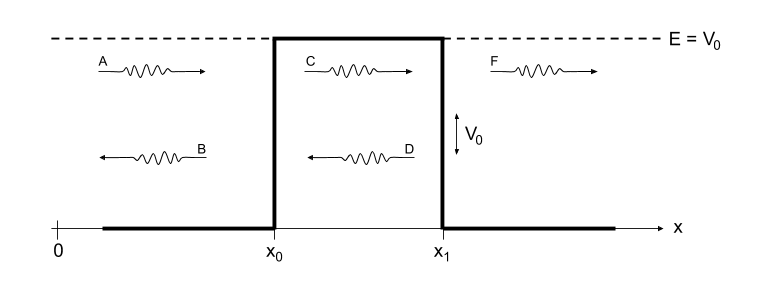
\includegraphics[width=0.6\textwidth]{potentialbarriere}
\caption{Potential barriere as given in the problem.}
\label{fig:figure_label}
\end{figure}


\subsubsection*{c.}

\begin{figure}[t]
\centering
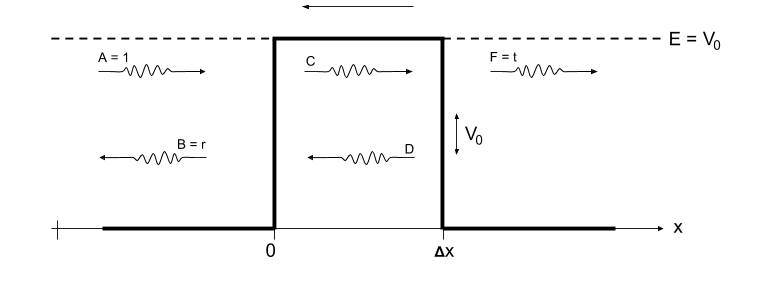
\includegraphics[width=0.6\textwidth]{potentialbarriereoffset}
\caption{To find boundary conditions, we offset the potential barriere by $-x_1$. We also set $A=1$, the \textit{incomming wave}, $B=r$, the \textit{reflected wave} and $F=t$, the \textit{transmitted wave}.}
\label{fig:figure_label}
\end{figure}

We need to look at the bounadary conditions for $\psi(x)$ and $d\psi/dx$. The derivatives of $\psi$ will have the following form

\begin{equation}
\frac{d\psi(x)}{dx} = \begin{cases}
ik(Ae^{ikx} - Be^{-ikx}) \ \ &, \ \ 0 \leq x \leq x_1 \\
q(Ce^{\kappa x} + De^{-\kappa x}) \ \ &, \ \ x_1 \leq x \leq x_e \\
ikFe^{ikx}  &, \ \ x \geq x_1 \\
\end{cases}
\end{equation}

Because the barriere is not located at $x=0$, we need to offset it by $-x_1$ which will give the following boundary conditions

\begin{align}
\psi_1(0) &= \psi_2(0), \\
\psi_2(\Delta x) &= \psi_3(\Delta x),\\
\frac{d}{dx}\psi_1(0) &= \frac{d}{dx}\psi_2(0) \ \text{and} \\
\frac{d}{dx}\psi_2(\Delta x) &= \frac{d}{dx}\psi_3(\Delta x), \\
\end{align}

which will give

\begin{align}
1 + r &= C + D, \label{eq_1} \\
Ce^{q\Delta x} + De^{-q\Delta x} &= t, \label{eq_2} \\
ik(1-r) &= q(C - D) \ \text{and} \label{eq_3} \\
q(Ce^{q\Delta x} - De^{-q\Delta x}) &= ikte^{ik\Delta x}, \label{eq_4} \\
\end{align}

where I have set $A = 1$, the \textit{incomming wave}, $B = r$, the \textit{reflected wave} and  $F = t$, the \textit{transmitted wave}.

Now we are left with four equations. We need to solve for $t$. This is straight forward and left as an exercice to the reader as it is trivial (I'm just kidding! Here it is!).

We start with (\ref{eq_2}), solving for $C$

\begin{equation}
C = \frac{te^{ik\Delta x}-De^{-q\Delta x}}{e^{q\Delta x}} \label{eq_5}
\end{equation}

Inserting (\ref{eq_5}) into (\ref{eq_4}) yields

\begin{equation}
q(te^{ik\Delta x} - 2De^{-q\Delta x}) = ikte^{ik\Delta x}.
\end{equation}

Solving for $t$ yields

\begin{equation}
    t = \frac{2qDe^{-z\Delta x}}{z^*}, \label{eq_6}
\end{equation}

where we have introduced the variables $z \equiv q + ik$ and $q^* \equiv q - ik$.

Next, eliminate $r$ from (\ref{eq_1}) and (\ref{eq_3}) to get

\begin{equation}
ik(1 - r) = q(C - D),
\end{equation}

which after some manipulations yields

\begin{equation}
C = \frac{Dz^* + 2ik}{z} \label{eq_7}.
\end{equation}

Setting (\ref{eq_5}) = (\ref{eq_7}) yields

\begin{equation}
te^{-z^*\Delta x} - De^{-2q\Delta x} = \frac{Dz^* + 2ik}{z},
\end{equation}

wich gives, by solving for $D$

\begin{equation}
D = \frac{tze^{-z^*\Delta x} - 2ik}{z^* + ze^{-2q\Delta x}} \label{eq_8}.
\end{equation}

Put (\ref{eq_8}) into (\ref{eq_6})

\begin{equation}
tz^* = \frac{tze^{-z^*\Delta x} - 2ik}{z^* + ze^{-2q\Delta x}}e^{-z\Delta x}
\end{equation}

which, if we solve for $t$ yields

\begin{align}
t &= \frac{2ike^{-z\Delta x}}{ze^{-(z^* + z)\Delta x} - \frac{z^*}{2q}(z^*+ze^{-2q\Delta x})} \\
  &= \frac{1}{\frac{ze^{-z^*\Delta x}}{2ik} - \frac{z^*e^{-z\Delta x}}{4ikq}(z^* + ze^{-2q\Delta x})}
\end{align}

$T = |t|^2$ and thus

\begin{equation}
T = \bigg( \frac{1}{\frac{ze^{-z^*\Delta x}}{2ik} - \frac{z^*e^{-z\Delta x}}{4ikq}(z^* + ze^{-2q\Delta x})} \bigg)^2
\end{equation}

I have skipped many steps, however, my calculations by hand is attached at the end of the document.

\subsubsection*{d.}

\subsubsection*{e.}

\subsubsection*{f.}

\subsubsection*{g.}


\end{document}

